\documentclass{standalone}
\usepackage{tikz}
\usetikzlibrary{patterns, positioning}
\usepackage[sfdefault]{ClearSans} %% option 'sfdefault' activates Clear Sans as the default text font
\usepackage[T1]{fontenc}

\begin{document}
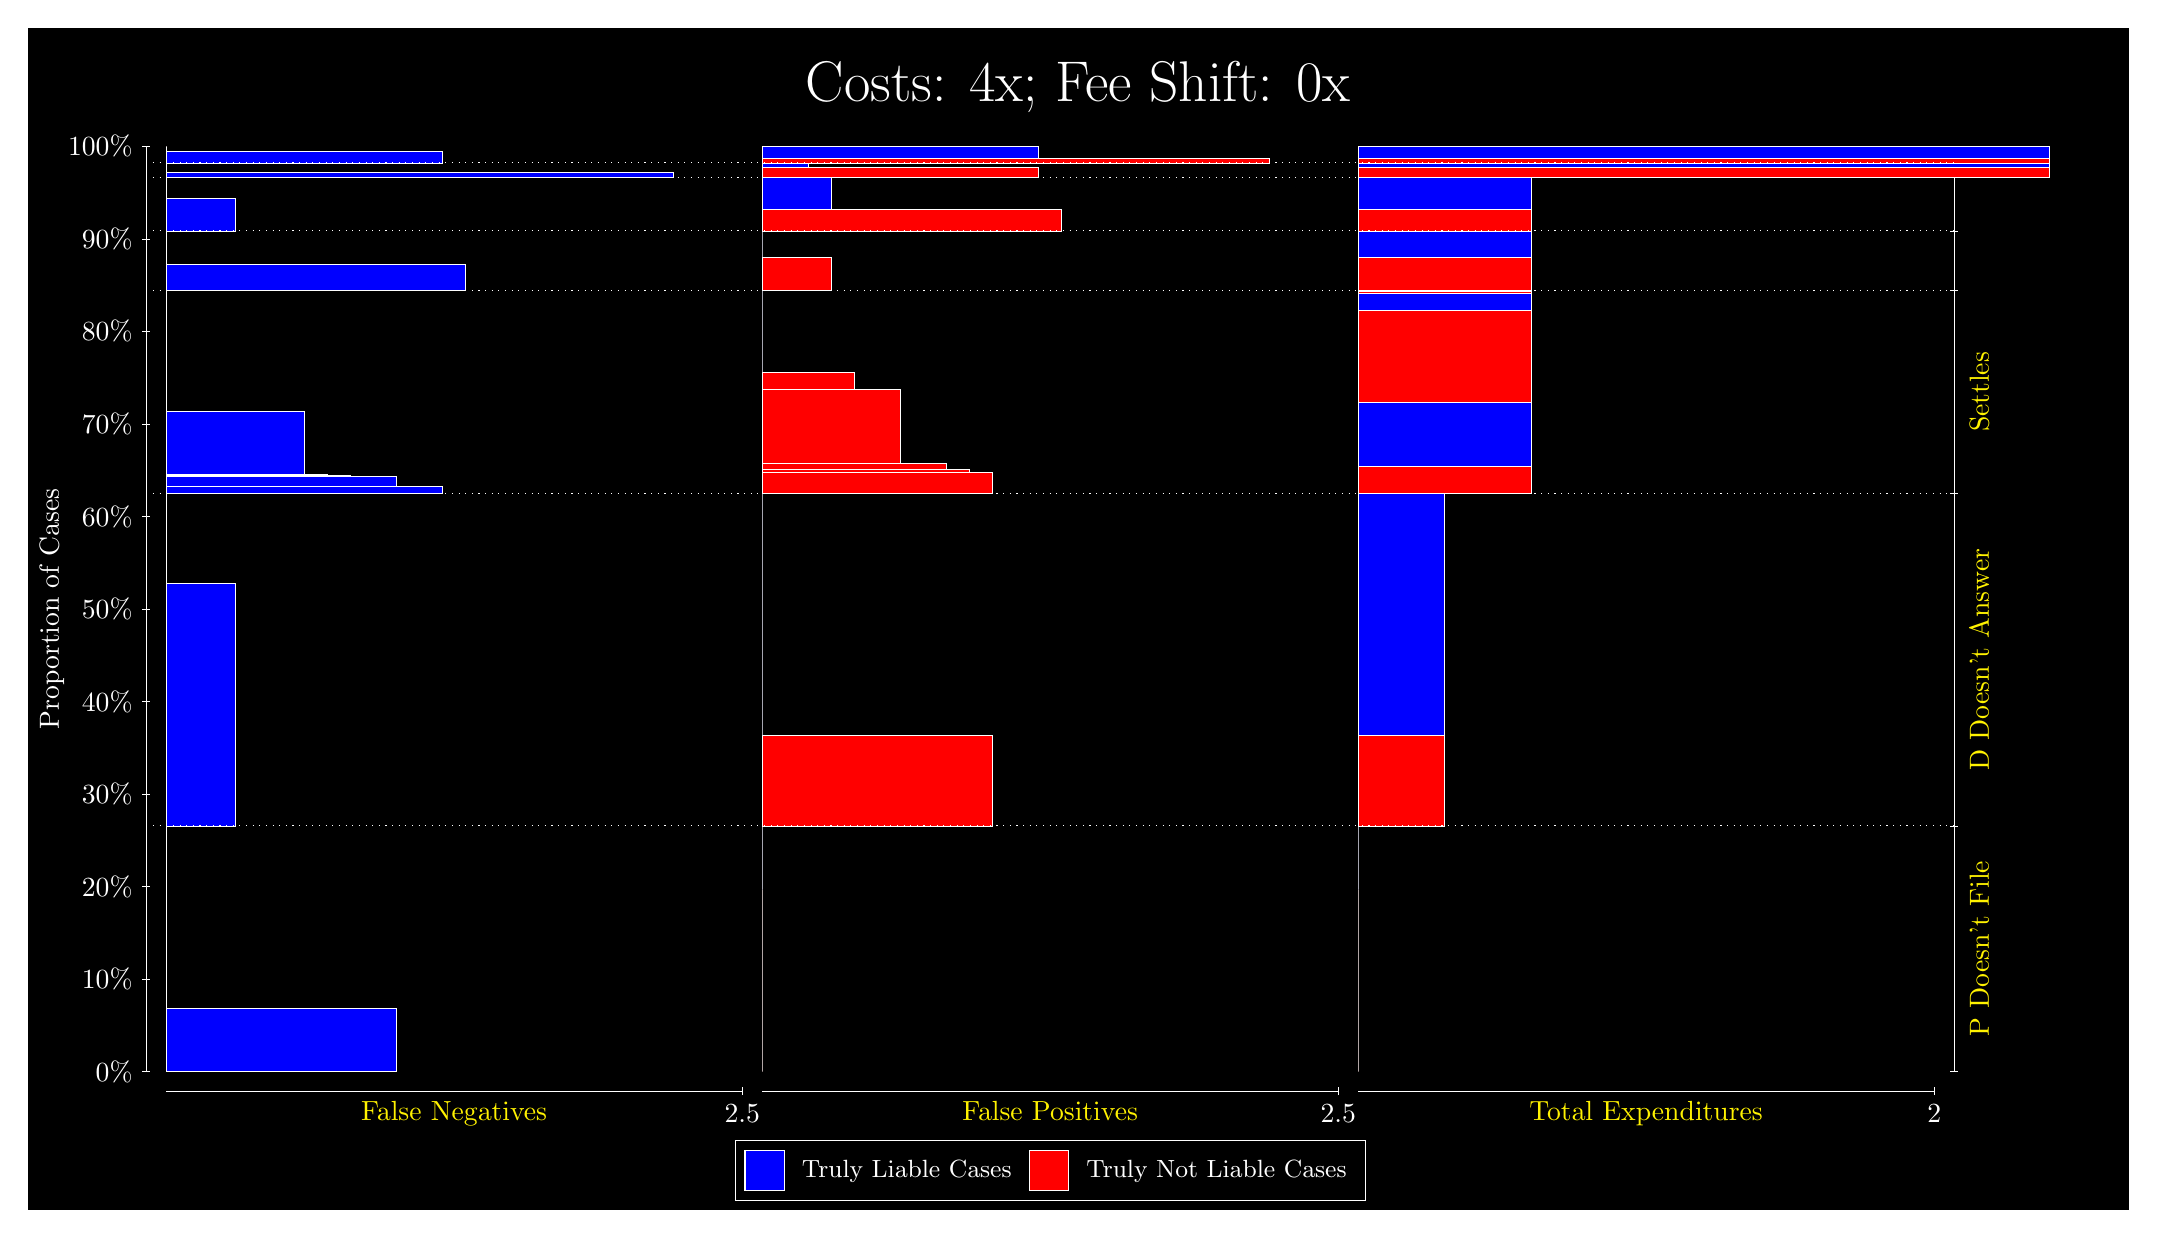
\begin{tikzpicture}
\draw[fill=black] (0,0) rectangle (26.667,15);
\draw[text=white] (0,13.5) rectangle (26.667,15) node[midway] {\huge Costs: 4x; Fee Shift: 0x};
\draw[white, very thin] (1.5,1.75) -- (1.5,13.5);
\node[rotate=90, text=white, anchor=center] at (0.3, 7.625) {Proportion of Cases};
\draw[white, very thin] (1.45,1.75) -- (1.55,1.75);
\node[text=white, anchor=east] at (1.45, 1.75) {0\%};
\draw[white, very thin] (1.45,2.925) -- (1.55,2.925);
\node[text=white, anchor=east] at (1.45, 2.925) {10\%};
\draw[white, very thin] (1.45,4.1) -- (1.55,4.1);
\node[text=white, anchor=east] at (1.45, 4.1) {20\%};
\draw[white, very thin] (1.45,5.275) -- (1.55,5.275);
\node[text=white, anchor=east] at (1.45, 5.275) {30\%};
\draw[white, very thin] (1.45,6.45) -- (1.55,6.45);
\node[text=white, anchor=east] at (1.45, 6.45) {40\%};
\draw[white, very thin] (1.45,7.625) -- (1.55,7.625);
\node[text=white, anchor=east] at (1.45, 7.625) {50\%};
\draw[white, very thin] (1.45,8.8) -- (1.55,8.8);
\node[text=white, anchor=east] at (1.45, 8.8) {60\%};
\draw[white, very thin] (1.45,9.975) -- (1.55,9.975);
\node[text=white, anchor=east] at (1.45, 9.975) {70\%};
\draw[white, very thin] (1.45,11.15) -- (1.55,11.15);
\node[text=white, anchor=east] at (1.45, 11.15) {80\%};
\draw[white, very thin] (1.45,12.325) -- (1.55,12.325);
\node[text=white, anchor=east] at (1.45, 12.325) {90\%};
\draw[white, very thin] (1.45,13.5) -- (1.55,13.5);
\node[text=white, anchor=east] at (1.45, 13.5) {100\%};

\draw[white, very thin] (24.457,1.75) -- (24.457,13.5);
\draw[white, very thin] (24.407,1.75) -- (24.507,1.75);
\node[anchor=west] at (24.407, 1.75) {};
\draw[white, very thin] (24.407,4.8694) -- (24.507,4.8694);
\node[anchor=west] at (24.407, 4.8694) {};
\draw[white, very thin] (24.407,9.0916) -- (24.507,9.0916);
\node[anchor=west] at (24.407, 9.0916) {};
\draw[white, very thin] (24.407,11.672) -- (24.507,11.672);
\node[anchor=west] at (24.407, 11.672) {};
\draw[white, very thin] (24.407,12.426) -- (24.507,12.426);
\node[anchor=west] at (24.407, 12.426) {};
\draw[white, very thin] (24.407,13.108) -- (24.507,13.108);
\node[anchor=west] at (24.407, 13.108) {};
\draw[white, very thin] (24.407,13.291) -- (24.507,13.291);
\node[anchor=west] at (24.407, 13.291) {};
\draw[white, very thin] (24.407,13.5) -- (24.507,13.5);
\node[anchor=west] at (24.407, 13.5) {};

\draw[white, very thin, fill=blue] (1.75,1.75) rectangle (4.6775,2.5577);
\draw[white, very thin, fill=red] (1.75,2.5577) rectangle (1.75,4.8694);
\draw[white, very thin, fill=blue] (1.75,4.8694) rectangle (2.6283,7.9467);
\draw[white, very thin, fill=red] (1.75,7.9467) rectangle (1.75,9.0916);
\draw[white, very thin, fill=blue] (1.75,9.0916) rectangle (5.2631,9.1875);
\draw[white, very thin, fill=blue] (1.75,9.1875) rectangle (4.6775,9.3045);
\draw[white, very thin, fill=blue] (1.75,9.3045) rectangle (4.092,9.3227);
\draw[white, very thin, fill=blue] (1.75,9.3227) rectangle (3.7993,9.338);
\draw[white, very thin, fill=blue] (1.75,9.338) rectangle (3.5065,10.132);
\draw[white, very thin, fill=red] (1.75,10.132) rectangle (1.75,11.672);
\draw[white, very thin, fill=blue] (1.75,11.672) rectangle (5.5558,12.005);
\draw[white, very thin, fill=red] (1.75,12.005) rectangle (1.75,12.426);
\draw[white, very thin, fill=blue] (1.75,12.426) rectangle (2.6283,12.834);
\draw[white, very thin, fill=red] (1.75,12.834) rectangle (1.75,13.108);
\draw[white, very thin, fill=blue] (1.75,13.108) rectangle (8.1906,13.165);
\draw[white, very thin, fill=red] (1.75,13.165) rectangle (1.75,13.291);
\draw[white, very thin, fill=blue] (1.75,13.291) rectangle (5.2631,13.443);
\draw[white, very thin, fill=red] (1.75,13.443) rectangle (1.75,13.5);
\draw[white, very thin, fill=red] (9.3189,1.75) rectangle (9.3189,4.0617);
\draw[white, very thin, fill=blue] (9.3189,4.0617) rectangle (9.3189,4.8694);
\draw[white, very thin, fill=red] (9.3189,4.8694) rectangle (12.246,6.0143);
\draw[white, very thin, fill=blue] (9.3189,6.0143) rectangle (9.3189,9.0916);
\draw[white, very thin, fill=red] (9.3189,9.0916) rectangle (12.246,9.3664);
\draw[white, very thin, fill=red] (9.3189,9.3664) rectangle (11.954,9.3939);
\draw[white, very thin, fill=red] (9.3189,9.3939) rectangle (11.661,9.4697);
\draw[white, very thin, fill=red] (9.3189,9.4697) rectangle (11.075,10.41);
\draw[white, very thin, fill=red] (9.3189,10.41) rectangle (10.49,10.632);
\draw[white, very thin, fill=blue] (9.3189,10.632) rectangle (9.3189,11.672);
\draw[white, very thin, fill=red] (9.3189,11.672) rectangle (10.197,12.093);
\draw[white, very thin, fill=blue] (9.3189,12.093) rectangle (9.3189,12.426);
\draw[white, very thin, fill=red] (9.3189,12.426) rectangle (13.125,12.7);
\draw[white, very thin, fill=blue] (9.3189,12.7) rectangle (10.197,13.108);
\draw[white, very thin, fill=red] (9.3189,13.108) rectangle (12.832,13.234);
\draw[white, very thin, fill=blue] (9.3189,13.234) rectangle (9.9044,13.291);
\draw[white, very thin, fill=red] (9.3189,13.291) rectangle (15.759,13.348);
\draw[white, very thin, fill=blue] (9.3189,13.348) rectangle (12.832,13.5);
\draw[white, very thin, fill=red] (16.888,1.75) rectangle (16.888,4.0617);
\draw[white, very thin, fill=blue] (16.888,4.0617) rectangle (16.888,4.8694);
\draw[white, very thin, fill=red] (16.888,4.8694) rectangle (17.986,6.0143);
\draw[white, very thin, fill=blue] (16.888,6.0143) rectangle (17.986,9.0916);
\draw[white, very thin, fill=red] (16.888,9.0916) rectangle (19.083,9.4422);
\draw[white, very thin, fill=blue] (16.888,9.4422) rectangle (19.083,10.254);
\draw[white, very thin, fill=red] (16.888,10.254) rectangle (19.083,11.417);
\draw[white, very thin, fill=blue] (16.888,11.417) rectangle (19.083,11.63);
\draw[white, very thin, fill=red] (16.888,11.63) rectangle (19.083,11.657);
\draw[white, very thin, fill=blue] (16.888,11.657) rectangle (19.083,11.672);
\draw[white, very thin, fill=red] (16.888,11.672) rectangle (19.083,12.093);
\draw[white, very thin, fill=blue] (16.888,12.093) rectangle (19.083,12.426);
\draw[white, very thin, fill=red] (16.888,12.426) rectangle (19.083,12.7);
\draw[white, very thin, fill=blue] (16.888,12.7) rectangle (19.083,13.108);
\draw[white, very thin, fill=red] (16.888,13.108) rectangle (25.67,13.234);
\draw[white, very thin, fill=blue] (16.888,13.234) rectangle (25.67,13.291);
\draw[white, very thin, fill=red] (16.888,13.291) rectangle (25.67,13.348);
\draw[white, very thin, fill=blue] (16.888,13.348) rectangle (25.67,13.5);
\draw[white, dotted] (1.5,4.8694) -- (24.457,4.8694);
\draw[white, dotted] (1.5,9.0916) -- (24.457,9.0916);
\draw[white, dotted] (1.5,11.672) -- (24.457,11.672);
\draw[white, dotted] (1.5,12.426) -- (24.457,12.426);
\draw[white, dotted] (1.5,13.108) -- (24.457,13.108);
\draw[white, dotted] (1.5,13.291) -- (24.457,13.291);
\draw[white, very thin] (1.75,1.5) -- (9.0689,1.5);
\node[text=yellow, anchor=north] at (5.4094, 1.5) {False Negatives};
\draw[white, very thin] (9.0689,1.45) -- (9.0689,1.55);
\node[text=white, anchor=north] at (9.0689, 1.45) {2.5};

\draw[white, very thin] (9.3189,1.5) -- (16.638,1.5);
\node[text=yellow, anchor=north] at (12.978, 1.5) {False Positives};
\draw[white, very thin] (16.638,1.45) -- (16.638,1.55);
\node[text=white, anchor=north] at (16.638, 1.45) {2.5};

\draw[white, very thin] (16.888,1.5) -- (24.207,1.5);
\node[text=yellow, anchor=north] at (20.547, 1.5) {Total Expenditures};
\draw[white, very thin] (24.207,1.45) -- (24.207,1.55);
\node[text=white, anchor=north] at (24.207, 1.45) {2};

\node[text=yellow, centered, rotate=90] at (24.777, 3.3097) {P Doesn't File};
\node[text=yellow, centered, rotate=90] at (24.777, 6.9805) {D Doesn't Answer};
\node[text=yellow, centered, rotate=90] at (24.777, 10.382) {Settles};





\draw (12.978300999999998,1.5) node[draw=none] (baseCoordinate) {};
\begin{scope}[align=center]
        \matrix[scale=0.5, draw=white, below=0.5cm of baseCoordinate, nodes={draw}, column sep=0.1cm]{
            \node[rectangle, draw, minimum width=0.5cm, minimum height=0.5cm, fill=blue] {}; &
            \node[draw=none, font=\small, text=white] (B) {Truly Liable Cases}; &
            \node[rectangle, draw, minimum width=0.5cm, minimum height=0.5cm, fill=red] {}; &
            \node[draw=none, font=\small, text=white] (B) {Truly Not Liable Cases}; \\
            };
\end{scope}

\end{tikzpicture}
\end{document}